\section{Aplikacja}
Celem tego rozdziału jest opisanie praktycznych efektów pracy, czyli
aplikacji \emph{Facjator}, której przeznaczeniem jest umożliwienie tworzenia
gramatyki kształtu oraz przetworzenie tej gramatyki na trójwymiarowy model.

Aplikacja kliencka to samodzielny program dostępny w dwóch wersjach,
umożliwiających działanie na platformie Windows oraz Linux.

\subsection{Organizacja aplikacji}
Aplikacja została napisana w języku C++ przy wykorzystaniu środowiska
deweloperskiego Visual C++ 2008 (dla systemów Windows) oraz środowiska Code
Blocks (dla systemów z rodziny Linux). Projekt składa się z katalogu z plikami
źródłowymi oraz plikami projektu dla Visual C++ 2008. 
W projekcie wykorzystywanych jest kilka bibliotek zewnętrznych:
\begin{enumerate}
  \item Lua\footnote{\url{http://www.lua.org - język skryptowy}};
  \item toLua++\footnote{\url{http://www.codenix.com/~tolua/}};
  \item FLTK 1.1\footnote{\url{http://www.fltk.org/}};
  \item
  VisualizationLibrary\footnote{\url{http://www.visualizationlibrary.com/jetcms/}}.
\end{enumerate}
Lua jest to język skryptowy, który w bardzo prosty sposób można zintegrować z
natywnymi programami napisanymi w języku C++. Język charakteryzuje się wysoką
wydajnością oraz prostą składnią, dzięki czemu można w krótkim czasie opanować
składnię na tyle, aby pisać proste programy. Podstawowa znajomość składni jest
niezbędna dla projektanta gramatyki kształtu, ponieważ gramatyka w programie
jest definiowana w języku Lua. Razem z Lua wykorzystujemy w programie bibliotekę
pomocniczą toLua++, której zadaniem jest uproszczenie komunikacji pomiędzy
programem a wykonywanymi skryptami poprzez eksportowanie klas do Lua. Do
utworzenia interfejsu została wykorzystana biblioteka FLTK w wersji 1.1.
VisualizationLibrary to biblioteka, która upraszcza dodanie do aplikacji
funkcjonalności wyświetlania grafiki dwu i trójwymiarowej. Tworzy ona cienką
warstwę pośredniczącą pomiędzy programem a biblioteką OpenGL.

Kompilacja projektu jest zależna od systemu, na którym projekt jest budowany. Na
systemie Windows wymagane jest środowisko Visual C++ w wersji 2008, wersja
Express jest udostępniana za
darmo\footnote{\url{http://www.microsoft.com/visualstudio/en-us/products/2008-editions/express}}.
Kompilacja sprowadza się do wczytania projektu \emph{facjator.sln} i
uruchomieniu procesu budowania aplikacji (domyślnie skrót F7). W rezultacie
tworzony jest plik wykonywalny \emph{facjator.exe}.
W przypadku systemu Linux najwygodniejszą metodą kompilacji aplikacji jest
wczytanie projektu \emph{face.cbp} w środowisku
Code::Blocks\footnote{\url{http://www.codeblocks.org/}} również dostępnego za
darmo i rozpoczęcia procesu kompilacji wraz z budowaniem (skrót F9). Należy
również pamiętać, aby w systemie były dostępne wyżej wymienione biblioteki.

\subsection{Architektura aplikacji}
Proces generowania trójwymiarowego modelu składa się z kilku następujących po
sobie etapów:
\begin{enumerate}
  \item Utworzenie nowej gramatyki kształtu bądź wczytanie istniejącej gramatyki
  z pliku projektu zapisanego na dysku (wykonuje użytkownik);
  \item Utworzenie bądź aktualizacja parametrów w przypadku, gdy gramatyka
  zawiera parametry (wykonuje użytkownik);
  \item Parsowanie gramatyki kształtu i przetworzenie jej przy użyciu jednego z
  dwóch istniejących algorytmów (przetwarzanie w przestrzeni wokselowej lub
  raytracing);
  \item Utworzenie trójwymiarowej reprezentacji modelu i wyświetlenie jej w
  oknie programu.
\end{enumerate}
Zasady tworzenia gramatyki zostaną opisane w dalszej części pracy. W kolejnych
akapitach skupimy się na opisie algorytmów i mechanizmów wykorzystywanych przez
aplikację.
\subsubsection{Reprezentacja gramatyki jako modelu trójwymiarowego}
Przed przesłaniem obiektów trójwymiarowych do karty graficznej w celu ich
wyrenderowania, konieczne jest przetworzenie ich na listę trójkątów. Jednak
zanim to nastąpi, można wykorzystać dowolną metodę opisu struktury geometrii w
zależności od tego, która jest najbardziej przydatna w konkretnym zastosowaniu.
Wybór ostatecznie wykorzystywanej reprezentacji jest bardzo istotny ze względu na to, że determinuje sposób definiowania gramatyki oraz parametryzacji kształtu.
Wybór reprezentacji geometrii trójwymiarowej został ograniczony do trzech
znanych nam metod:
\begin{enumerate}
  \item Siatka trójkątów bądź czworoboków (zobacz ~\ref{fig:rep_geom1});
  \item Powierzchnie parametryczne (przy czym brano pod uwagę głównie
  hierarchiczne b-splajny, zobacz~\ref{fig:rep_geom2});
  \item Reprezentacja przy użyciu ograniczonej liczby dowolnych elementarnych
  obiektów, które mają swoją matematyczną reprezentację i przetwarzaniu takiej
  struktury w przestrzeni wokselowej lub przy użyciu algorytmu śledzenia
  promieni (ang. raytracing).
\end{enumerate}

{
\begin{figure}[h]
  \centering
  \subfloat[Siatka
  wielokątów.]{\label{fig:rep_geom1}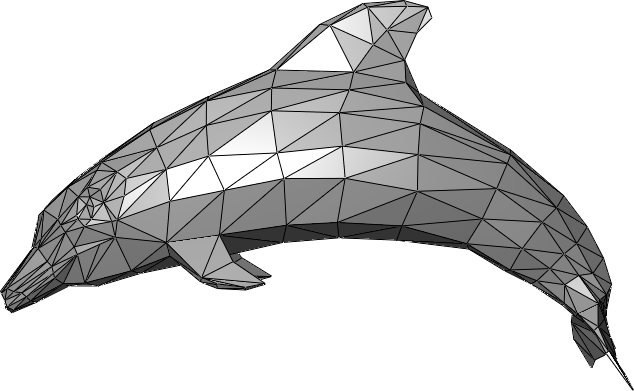
\includegraphics[width=6cm]{images/triangle_mesh.png}}
  \quad
  \subfloat[Hierarchiczne
  B-Splajny]{\label{fig:rep_geom2}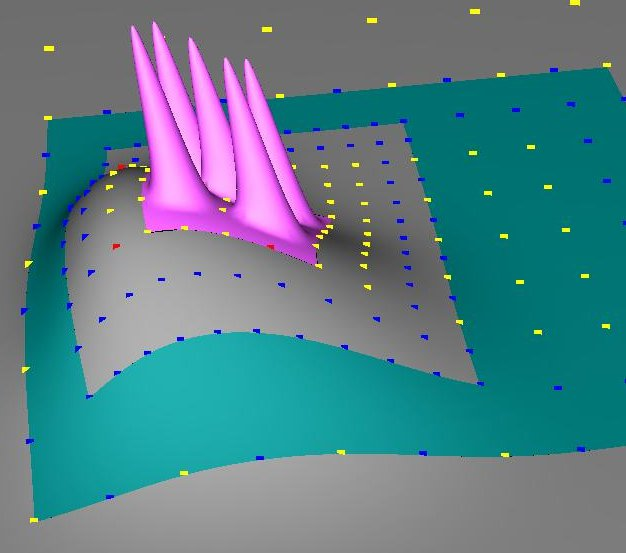
\includegraphics[width=6cm]{images/hspline.jpg}}
  \quad
  \label{fig:rep_geom}
  \caption{Reprezentacje geometrii~$^{\decimal{footnote}}$.}
\end{figure}
\footnotetext[\value{footnote}]{\url{http://en.wikipedia.org/wiki/File:Dolphin_triangle_mesh.png},
\url{http://www.cgl.uwaterloo.ca/~ecdfourq/courses/cs779/project.html}}
}

Reprezentacja za pomocą siatki wielokątów\cite{link11}\cite{link12} jest
najprostszym ze sposobów reprezentacji modelu trójwymiarowego. Dodatkowo jest to
również format, w którym dane można przesyłać do karty graficznej, więc gdy
chcemy taką siatkę wyświetlić to z reguły nie jest wymagana żadna dodatkowa
konwersja. Siatka wielokątów~\ref{vef_image} w kontekście grafiki trójwymiarowej to
zbiór kilku elementów:
\begin{enumerate}
  \item wierzchołków, które są podstawowymi elementami definiującymi położenie
  punktów budujących model. Może być dowolnie wiele wierzchołków i same w sobie
  nie są wystarczające do tego, aby określić budowę modelu. Z wierzchołkami
  najczęściej powiązane są inne dane, takie jak --- kolor, współrzędne u,v dla
  tekstury nałożonej na siatkę oraz wektor normalny wykorzystywany do wyliczenia
  oświetlenia. Z perspektywy naszego programu dane te nie są istotne więc
  zostaną pominięte;
  \item krawędzi, które są zdefiniowane jako para dwóch wierzchołków, bez
  dodatkowych informacji;
  \item wielokątów (ang. face), które łączą krawędzie w grupy tworząc
  strukturę modelu. \emph{Face} może być dowolnym wielokątem, ale najczęściej
  wykorzystywanymi są trójkąt i czworokąt z uwagi na prostotę takiego rozwiązania.
\end{enumerate}
Mając definicję wielokątów można bez problemów określić powiązania pomiędzy
wierzchołkami i przygotować dane akceptowalne przez kartę graficzną.
Ten sposób reprezentacji geometrii ma dużą zaletę z uwagi na dosyć prostą
możliwość modyfikacji geometrii. Ponieważ wierzchołki definiują położenie 
punktów modelu, to w najprostszych przypadkach wystarczy modyfikować ich
położenie. Nieco większy stopień komplikacji mają algorytmy do operacji
logicznych na siatkach (and. constructive solid geometry\footnote{Technika
tworzenia skomplikowanych modeli polegająca na wykonywaniu operacji logicznych
na innych modelach.}), ale jest to możliwe do osiągnięcia. Niewątpliwie minusem
jest ograniczona szczegółowość odwzorowania modelowanych obiektów, które są
zależne od wielkości używanych wielokątów. Najprostszym
rozwiązaniem jest zwiększenie ich ilości przy równoczesnym zmniejszeniu ich
rozmiarów, jednakże szybko geometria ta staje się ciężka w zarządzaniu i wymaga
dużych zasobów obliczeniowych.
{
\begin{figure}[h]
  \centering
  \subfloat{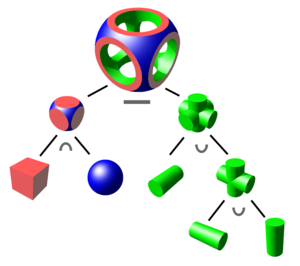
\includegraphics[width=6cm]{images/Csg.png}}
  \label{csg_image}
  \caption{Operacje CSG na modelach pozwalają tworzyć skomplikowane
  kształty~$^{\decimal{footnote}}$.}
\end{figure}
\footnotetext[\value{footnote}]{\url{http://en.wikipedia.org/wiki/Constructive_solid_geometry}}
}
\begin{figure}
\centering
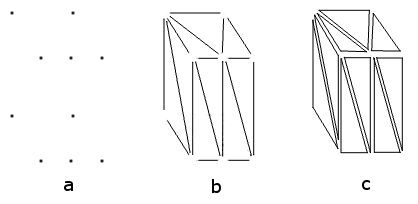
\includegraphics[width=8cm]{images/v_e_f.png}
\caption{Wierzchołki (a), krawędzie (b) oraz wielokąty (c) w modelu
trójwymiarowym (źródło własne).}
\label{vef_image}
\end{figure}

Główną wadą siatki wielokątów jest to, że przy jej użyciu ciężko modeluje się
gładkie powierzchnie. Do tego zadania o wiele lepiej nadaje się reprezentacja
geometrii za pomocą powierzchni parametrycznych. Rozwój prac nad powierzchniami
tego typu w grafice komputerowej zawdzięczamy w dużej mierze przemysłowi
motoryzacyjnemu, który potrzebował łatwego sposobu na tworzenie wizualizacji
samochodów i ich gładkich powierzchni.
W grafice często stosowane są powierzchnie
NURBS\footnote{http://en.wikipedia.org/wiki/Non-uniform\_rational\_B-spline}
(ang. Non-Uniform Rational B-Spline). Powierzchnia taka składa się z punktów kontrolnych, węzłów oraz wag punktów kontrolnych. Modyfikując te składowe parametry wpływa
się na wygląd powierzchni. Istotnym rozszerzeniem są powierzchnie typu
\emph{Hierarchical B-Spline} i możliwość dzielenia pojedynczego regionu zamiast
całej powierzchni. Daje to duże możliwości podczas modelowania obiektów, gdyż
pozwala na dodanie szczegółów tam, gdzie są niezbędne bez modyfikacji pozostałej
geometrii.
{
\begin{figure}[h]
  \centering
  \subfloat{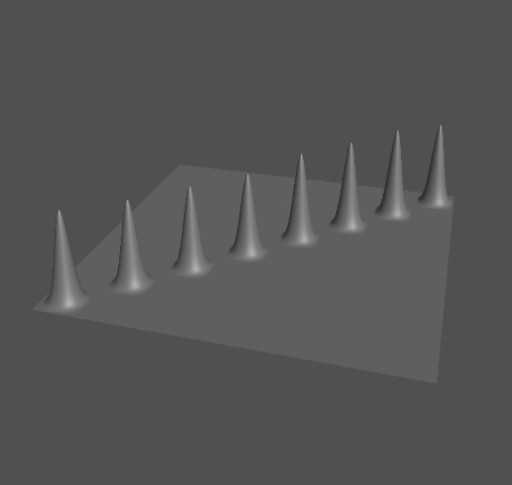
\includegraphics[width=5cm]{images/worstG.jpg}}
  \quad
  \subfloat{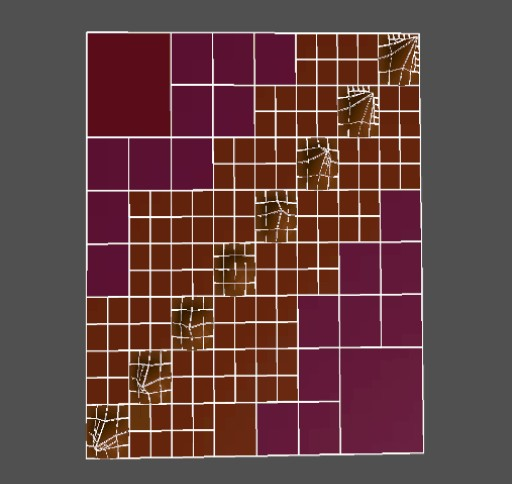
\includegraphics[width=5cm]{images/worstL.jpg}}
  \quad
  \label{fig:hbspline}
  \caption{Zmodyfikowana powierzchnia parametryczna z
  lokalnymi podziałami~$^{\decimal{footnote}}$.}
\end{figure}
\footnotetext[\value{footnote}]{\url{http://www.cs.ubc.ca/nest/imager/contributions/forsey/dragon/hbsplines.html}}
}

Reprezentacja wokselowa wyróżnia inne podejście do problemu tworzenia i
przechowywania w pamięci modelu trójwymiarowego. Zaprezentowane wcześniej
sposoby reprezentacji geometrii skupiały się na tworzeniu samej zewnętrznej
powłoki modelu, natomiast woksele zajmują również wewnętrzną przestrzeń modelu.
Przy wykorzystaniu tej techniki, od razu można zauważyć podatność na
zastosowanie różnego rodzaju algorytmów logicznych na wokselach, głównie ze względu na
prostotę implementacji w porównaniu do wcześniej opisanych reprezentacji
geometrii, zwłaszcza powierzchni parametrycznych. Podstawowym elementem w tej
reprezentacji jest woksel. Jest to obiekt w przestrzeni trójwymiarowej
reprezentujący wartość. Przestrzeń przechowująca woksele ma postać tablicy
trójwymiarowej, gdzie na pojedynczy element tablicy przypada jeden woksel. Dane przechowywane przez woksele mogą być dowolnej
postaci i zależą od zastosowania. W najprostszym przypadku może to być
pojedyncza flaga, oznaczająca czy dany woksel jest zajęty (renderowalny) czy
nie (przeźroczysty). Tworzenie kształtów polega w takim przypadku na włączaniu i
wyłączaniu odpowiednich wokseli. W związku z tym, że dane sa przechowywane w
formie dyskretnej, może pojawić się aliasing\footnote{W grafice komputerowej
jest to zjawisko polegające na zniekształceniu obrazu w wyniku zbyt małej częstości
próbkowania, objawia się widocznymi \emph{schodkami} w miejscu, gdzie powinny
był gładkie kształty.}. Częściowo można rozwiązać ten problem poprzez
zwiększenie liczby wokseli, jednak pociąga to za sobą zwiększone zapotrzebowanie
na zasoby obliczeniowe komputera. Do usunięcia aliasingu może się również
przyczynić algorytm użyty do renderowania obiektów wokselowych np. marching
cubes.

{
\begin{figure}[h]
  \centering
  \subfloat{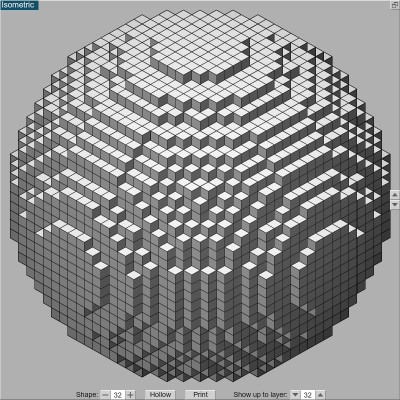
\includegraphics[width=5cm]{images/voxel_sphere.jpg}}
  \label{fig:voxel_sphere}
  \caption{Sfera wyświetlona jako obiekt wokselowy~$^{\decimal{footnote}}$.}
\end{figure}
\footnotetext[\value{footnote}]{\url{http://www.plotz.co.uk}}
}

\subsubsection{Parametryzacja geometrii}
Jednym z problemów związanych z geometryczną reprezentacją głowy jest
parametryzacja geometrii. Każdy z opisanych wcześniej sposobów reprezentacji
przy użyciu wielokątów najbardziej odpowiednie wydaje się
parametryzowanie położenia poszczególnych wierzchołków budujących strukturę
modelu. Możliwości wydają się nieograniczone, jednak dość łatwo można sobie
wyobrazić trudność polegającą na zachowaniu dobrego efektu wizualnego przy
próbie symulowania gładkich powierzchni. Rozwiązaniem może być zastosowanie
modyfikatorów proporcjonalnych (znanych z różnych programów służących do edycji
trójwymiarowych modeli), które są wykorzystywane do zachowania gładkości
modyfikowanej powierzchni. Z naszych prób wynika, że efekt może nie być
zadowalający przy dużym skomplikowaniu modelu. Biorąc pod uwagę modyfikatory proporcjonalne, dosyć trudne wydaje się wyizolowanie modyfikowanych wierzchołków, w sytuacji gdy blisko siebie znajdują się różne, niezależne powierzchnie. W przypadku powierzchni parametrycznych najlepszym sposobem parametryzacji jest
modyfikowanie punktów kontrolnych powierzchni. Powierzchnie tego typu zachowują swoją gładkość w przypadku zmiany parametrów,
co wydaje się być dużym plusem, biorąc pod uwagę charakter tworzonego przez nas
modelu. Można powiedzieć, że modyfikowane powierzchnie zachowywałyby
naturalność.

Tak jak w reprezentacji siatki do budowania modelu używa się wielokątów,
w reprezentacji parametrycznej hierachicznych b-splajnów, tak w reprezentacji
wokselowej podstawowym elementem jest pojedynczy woksel. Rozsądne wydaje się
przejście na wyższy poziom i budowanie modeli wykorzystując podstawowe
elementy, jak sfery, sześciany itp.. W kontekście parametryzacji oznacza,
że można poddawać modyfikacji parametry tych obiektów np. pozycję,
obrót, skalę. Przedstawione dotąd sposoby parametryzacji dotyczyły pojedynczych
elementów reprezentacji geometrycznych. Wydaje się jednak, że niezbędne jest również parametryzowanie w kontekście kilku elementów np. wykonywanie operacji logicznych. W każdej
reprezentacji jest to możliwe, jednak poziom komplikacji jest bardzo różny.
Biorąc pod uwagę nasze potrzeby zdecydowano, że zostanie wykorzystana
reprezentacja wokselowa. Duże znaczenie przy wyborze miała w miarę
bezproblemowa implementacja kilku operacji, którą później planowaliśmy
wykorzystać w tworzeniu i parametryzacji modelu.

\subsubsection{Przetwarzanie gramatyki w przestrzeni wokselowej}
Przetwarzanie gramatyki kształtu w przestrzeni wokselowej sprowadza się
do wykonania operacji tworzących drzewo gramatyki (ilustracja
~\ref{tree_traversal_algo}) na każdym wokselu. Każdy woksel ma unikalną
współrzędną, która wykorzystywana jest do sprawdzania poprawności w kontekście
wszystkich terminali i nieterminali.

\subsubsection{Ray-tracing}
Model matematycznego przechowywania geometrii zastosowany w pracy wpłynął na
zastosowanie w programie alternatywnego algorytmu renderowania:
ray-tracingu\footnote{\url{http://en.wikipedia.org/wiki/Ray\_tracing\_\%28graphics\%29}}.
O samej metodzie renderowania metodą ray-tracingu można znaleźć wiele materiałów
w sieci dlatego poniżej opisana zostanie jedynie implementacja w programie
\emph{Facjator}.

Mając reprezentacje matematyczną obiektów (pomijając fakturę obiektów), idea nie
różni się od klasycznej metody ray-tracingu -- najpierw wypuszczany jest promień
z pozycji kamery, kierowany jest do konkretnego piksela na płaszczyźnie
rzutowania i dalej rzutowany w przestrzeń. Następnie badane są przecięcia z
obiektami znajdującymi się na scenie. Jeżeli nastąpiła kolizja to wyliczamy
natężenie światła w punkcie trafienia na podstawie wektora normalnego do
powierzchni, wektora do kamery i wektora do światła; jeśli nie było trafienia,
ustawiany jest kolor czarny i cały proces jest powtarzany dla kolejnego piksela.
Istnieje tylko jedna sytuacja, w której klasyczna metoda zawiedzie,
zaprezentowana jest na ilustracji~\ref{ray_trace01}

\begin{figure}[h]
  \centering
  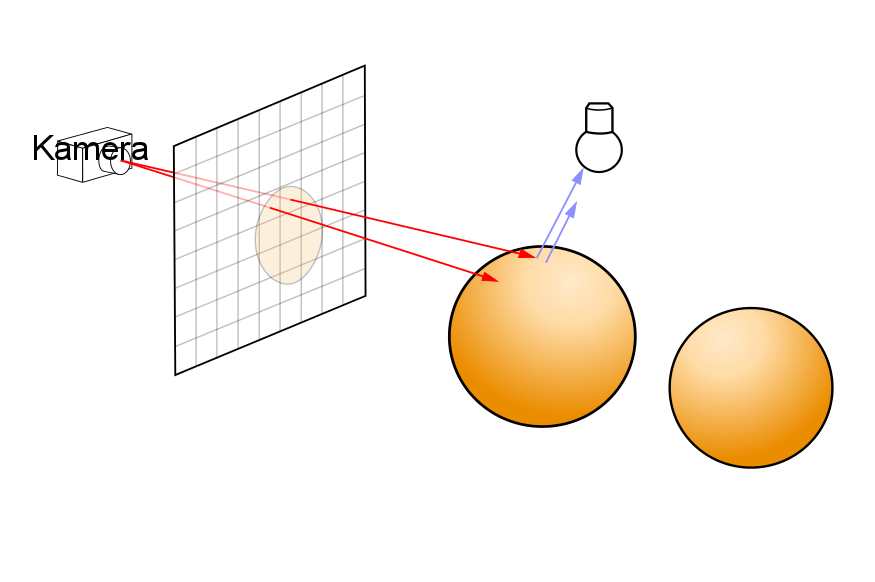
\includegraphics[width=12cm]{images/ray_trace01.png}
  \caption{Problem ray-tracingu i operacji boolowskich (źródło własne).}
  \label{ray_trace01}
\end{figure}

W przypadku klasycznego renderingu, informacja o drugim obiekcie jest tracona,
gdyż jest renderowany obiekt, który jest bliżej kamery (pierwsza kula
zakrywa drugą kulę, więc zostanie wyrenderowana tylko pierwsza kula).
Zakładając, że pierwsza kula zostaje wycięta ze sceny operacją {\em Diff} to
brak informacji o dalszym obiekcie spowoduje, że nie zostanie wyrenderowany
żaden obiekt (a powinien być drugi).

Aby rozwiązać ten problem została zaimplementowana taka metoda, która pozwoli
zapamiętać wszystkie obiekty na drodze promienia. W tym celu opracowano klasę
{\em set} reprezentującą zbiór odcinków, gdzie jeden odcinek reprezentuje obszar
wewnątrz obiektu (ilustracja~\ref{ray_trace02}).

\begin{figure}[h]
  \centering
  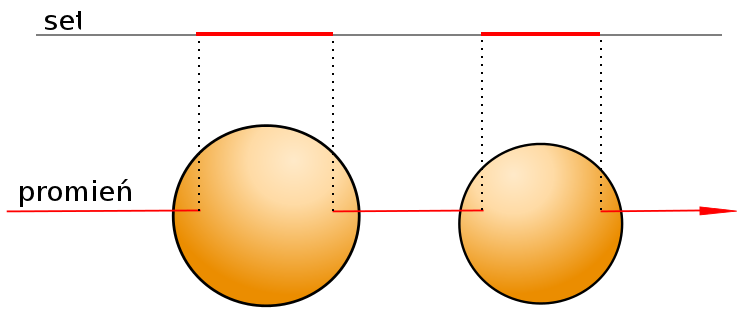
\includegraphics[width=12cm]{images/ray_trace02.png}
  \caption{Przykład zastosowania klasy {\em set} (źródło własne).}
  \label{ray_trace02}
\end{figure}
Dzięki użyciu klasy {\em set} operacje boolowskie sprowadzają się do operacji na
zbiorach odcinków (suma odcinków, różnica odcinków, część wspólna odcinków
itp.). Po wykonaniu wszystkich operacji na obiektach, wyciągany jest ze zbioru
element położony najbliżej kamery (minimum ze zbioru). Obiekt ten zostaje
wyrenderowany.

\begin{figure}[h]
  \centering
  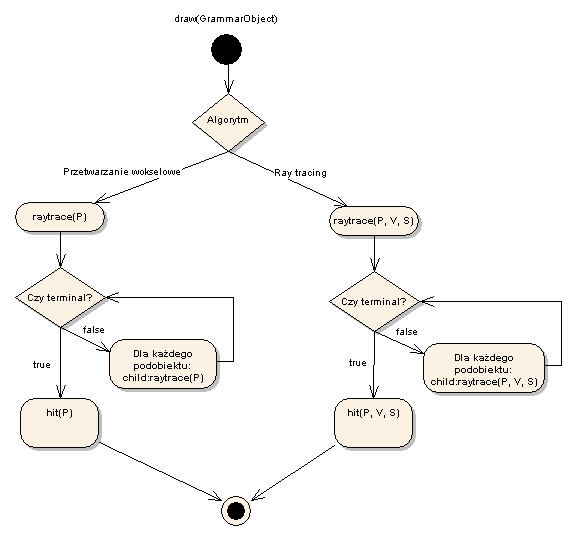
\includegraphics[width=12cm]{images/tree_traversal.PNG}
  \caption{Implementacja przetwarzania drzewa gramatyki kształtu (źródło
  własne).}
  \label{tree_traversal_algo}
\end{figure}

\subsubsection{Interfejs aplikacji}
Główne okno aplikacji składa się z kilku podokien o różnym przeznaczeniu.
Zgodnie z oznaczeniami na ilustracji~\ref{main_window} poszczególne elementy
okna to:
\begin{enumerate}
  \item menu aplikacji,
  \begin{enumerate}
    \item File-New - utworzenie nowego, pustego projektu;
    \item File-Open - okno wyboru pliku projektu do wczytania, istniejące
    parametry oraz skrypt gramatyki zostaną zastąpione;
    \item File-Save - zapisanie zmian w projekcie do aktywnego pliku na dysku;
    \item File-Save As - zapisanie aktualnego projektu do nowego pliku;
    \item Edit-Undo - cofnięcie ostatniej operacji edycji;
    \item Edit-Redo - ponowienie ostatniej operacji edycji;
    \item Edit-Cut - wycięcie zaznaczonego tekstu;
    \item Edit-Copy - kopiowanie zaznaczonego tekstu;
    \item Edit-Paste - wklejenie skopiowanego wcześniej tekstu;
  \end{enumerate}
  \item okno wyświetlające efekt końcowy przetwarzania gramatyki czyli gotowy
  model trójwymiarowy. Aby uaktywnić opcję orbitowania kamery wokół modelu
  należy kliknąć i przytrzymać prawy przycisk myszy w oknie oraz poruszać
  kursorem, zwolnienie przycisku wyłączy funkcję orbitowania (opcja dostępna
  tylko podczas przetwarzania gramatyki w przestrzeni wokselowej);
  \item okna pozwalające na wczytanie wzorcowych obrazów tworzonego modelu.
  Wciśnięcie prawego przycisku myszy wyświetla menu podręczne,
  \item edytor skryptu gramatyki;
  \item przyciski do wykonywania operacji:
  \begin{enumerate}
    \item przetwarzanie gramatyki w przestrzeni wokselowej (Compile);
    \item przetwarzanie gramatyki algorytmem śledzenia promieni (Ray trace);
    \item pole tekstowe do wprowadzania rozmiaru przestrzeni wokselowej oraz do
    aktualizacji tej wartości w projekcie (Update size);
    \item przycisk do przywracania domyślnych ustawień kamery (Reset camera);
    \item przyciski do ustawiania kamery z wybranej strony elementu: lewej
    (\emph{Left}), prawej (\emph{Right}), z góry (\emph{Top}), od dołu
    (\emph{Bottom}), od przodu (\emph{Front}), od tyłu (\emph{Back}).
  \end{enumerate}
  \item okno z listą zdefiniowanych parametrów oraz przyciskami umożliwiającymi
  dodawanie nowych, usuwanie, edycję istniejących parametrów.
\end{enumerate}

\begin{figure}[h]
  \centering
  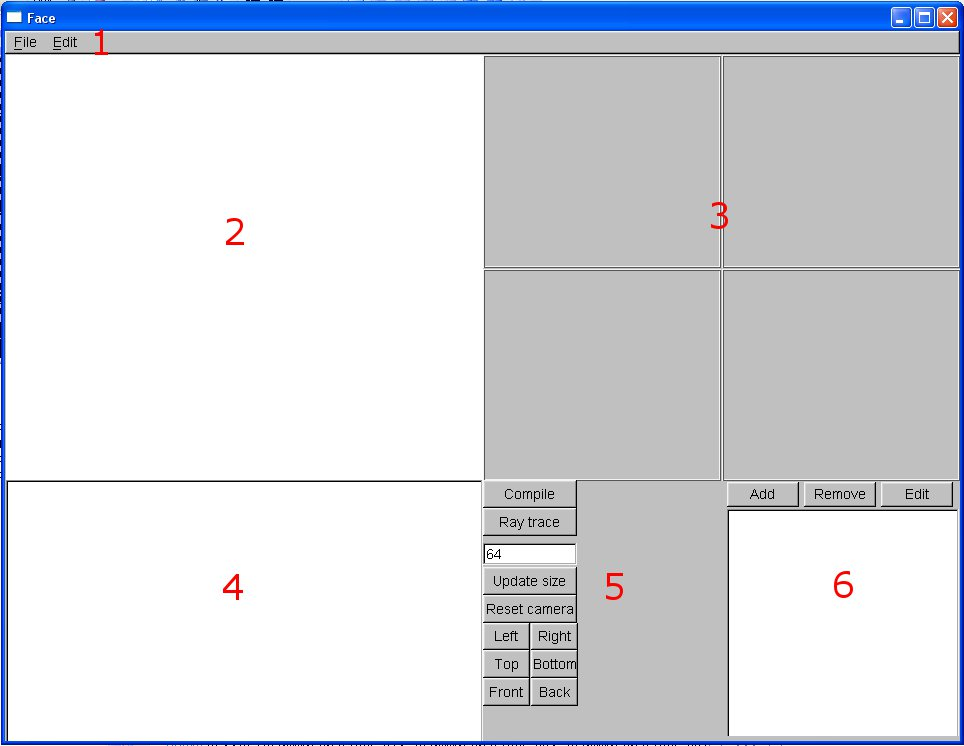
\includegraphics[width=0.7\textwidth]{images/ui.jpg}
  \caption{Główne okno aplikacji (źródło własne)}
  \label{main_window}
\end{figure}

\begin{figure}[h]
  \centering
  \subfloat{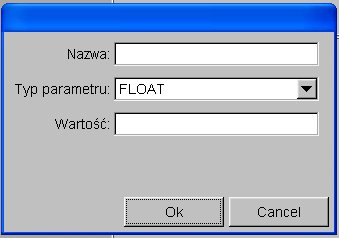
\includegraphics[width=5cm]{images/ui_def_param.jpg}}
  \caption{Okno definicji nowego parametru (źródło własne)}
  \label{new_param_window}
  \quad
  \subfloat{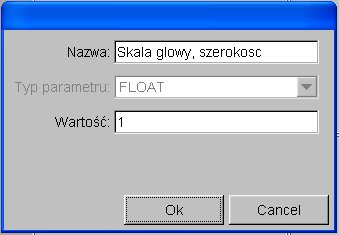
\includegraphics[width=5cm]{images/ui_edit_param.jpg}}
  \caption{Okno edycji istniejącego parametru (źródło własne)}
  \label{edit_param_window}
\end{figure}
Wybranie przycisku dodawania nowego parametru otwiera okno zaprezentowane na
ilustracji~\ref{new_param_window}. Można w nim wprowadzić unikalną nazwę
parametru opisującą jego funkcję, typ danych przechowywanych przez parametr oraz domyślną
wartość parametru. Zdefiniowane parametry można edytować zaznaczając je na
liście i wybierając przycisk edycji. Okno edycji przedstawione na
ilustracji~\ref{edit_param_window} pozwala na zmianę nazwy oraz wartości
parametru. Po utworzeniu parametru nie ma możliwości zmiany typu przechowywanych danych.
Z poziomu gramatyki kształtu do parametru odwołujemy się przy użyciu jego nazwy.

\subsubsection{Operacje oraz modyfikatory w gramatyce kształtu}
W zaimplementowanym programie zostało wykorzystanych kilka elementarnych obiektów oraz
modyfikatorów bazujących na technikach \emph{CSG}\footnote{ang. Constructive
Solid Geometry}. W tabelach~\ref{elements_table}, \ref{transforms_table},
\ref{operations_table}, \ref{misc_table} zostały przedstawione wszystkie
możliwości oraz przykłady wykorzystania modyfikatorów.

\setlength\fboxsep{2pt}
\setlength\fboxrule{0pt}
{
\noindent
\begin{center}
\begin{table}[hb]
\begin{tabular}{| p{0.55\textwidth} | p{0.35\textwidth} | }
  \hline
  \rowcolor{lightgray} Opis obiektu & Przykład użycia \\ \hline \hline
  
  \textbf{Sześcian}\newline
  Generuje model sześcianu o rozmiarach 2x2x2 &
  local cube = Cube(); \newline draw(cube); \\ \hline
  \multicolumn{2}{|c|}{\fbox{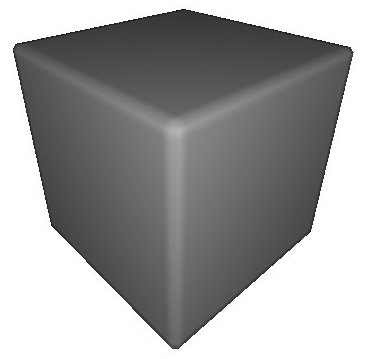
\includegraphics[width=4cm]{images/elem_cube.jpg}}}
  \\
  \hline
  
  \textbf{Sfera}\newline
  Generuje model sfery o promieniu równym 1 &
  local sphere = Sphere(); \newline draw(sphere); \\ \hline
  \multicolumn{2}{|c|}{\fbox{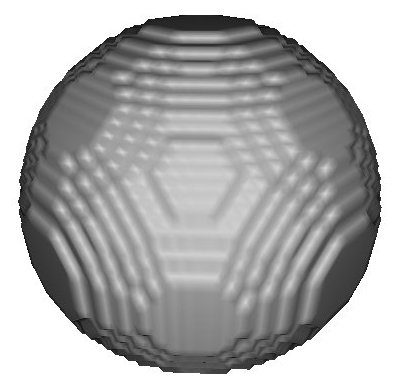
\includegraphics[width=4cm]{images/elem_sphere.jpg}}}
  \\
  \hline
\end{tabular}
\caption{Podstawowe modele (obiekty elementarne) dostępne w gramatyce kształtu
(źródło własne)}
\label{elements_table}
\end{table}
\end{center}
}

{
\noindent
\begin{center}
\begin{table}[hp]
\begin{tabular}{| p{0.55\textwidth} | p{0.35\textwidth} | }
  \hline
  \rowcolor{lightgray} Opis obiektu & Przykład użycia \\ \hline \hline  
  \textbf{Walec}
  \newline Generuje model walca kołowego prostego o promieniu podstawy równym 1
  oraz wysokości równej 2 &
  local cylinder = Cylinder(); \newline draw(cylinder); \\ \hline
  \multicolumn{2}{|c|}{\fbox{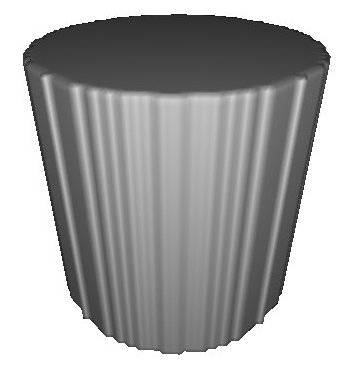
\includegraphics[width=4cm]{images/elem_cylinder.jpg}}}
  \\
  \hline
  
  \textbf{Stożek}
  \newline Generuje model stożka prostego o promieniu podstawy równym 1 oraz
  wysokości równej 1 & local cone = Cone(); \newline draw(cone); \\
  \hline
  \multicolumn{2}{|c|}{\fbox{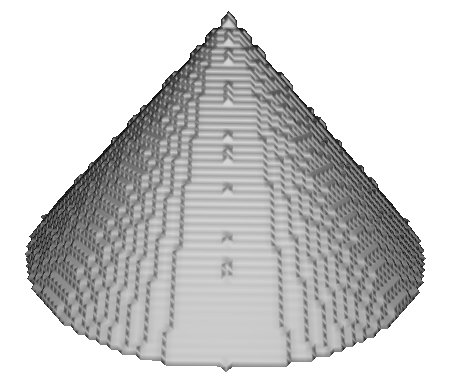
\includegraphics[width=4cm]{images/elem_cone.jpg}}}
  \\
  \hline

  \textbf{Torus}
  \newline Generuje torus o podanych promieniach. Pierwszy argument to promień
  torusa, drugi to promień okręgu tworzącego tunel & local torus = Torus(0.66,
  0.23); \newline draw(torus); \\ \hline
  \multicolumn{2}{|c|}{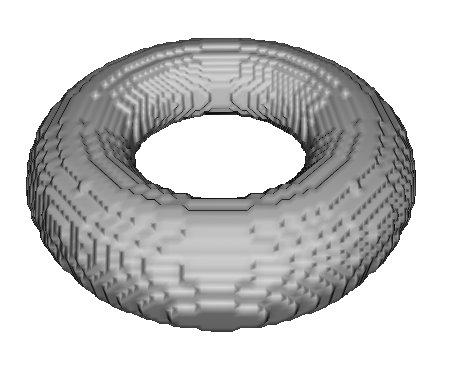
\includegraphics[width=4cm]{images/elem_torus.jpg}}
  \\
  \hline
\end{tabular}
\caption{Podstawowe modele (obiekty elementarne) dostępne w gramatyce kształtu
cd.}
\label{elements_table}
\end{table}
\end{center}
}

{
\noindent
\begin{center}
\begin{table}[hp]
\begin{tabular}{| p{0.55\textwidth} | p{0.35\textwidth} | }
  \hline
  \rowcolor{lightgray} Opis transformacji & Przykład użycia \\ \hline \hline
  
  \textbf{Translacja}\newline
  Przesuwa obiekt, na rzecz którego następuje wywołanie o wybrany wektor &
  local cube = Cube(); \newline cube:translate(0.5, 0, 0) \newline --
  przesunięcie o 0.5 jednostek wzdłuż osi X \\ \hline
  \multicolumn{2}{|c|}{\fbox{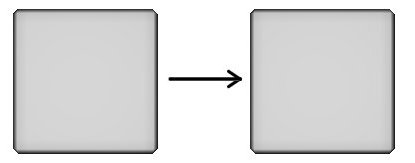
\includegraphics[width=8cm]{images/op_translate.jpg}}}
  \\
  \hline
  
  \textbf{Rotacja}\newline
  Obraca obiekt, na rzecz którego następuje wywołanie o kąt wokół osi X, Y i Z.
  Wartość kąta jest podawana w radianach (rotate) bądź stopniach (rotateDeg) &
  local cube = Cube(); \newline cube:rotateDeg(0.0, 0, 30.0) \newline --
  obrót o 30 stopni wokół osi Z \\ \hline
  \multicolumn{2}{|c|}{\fbox{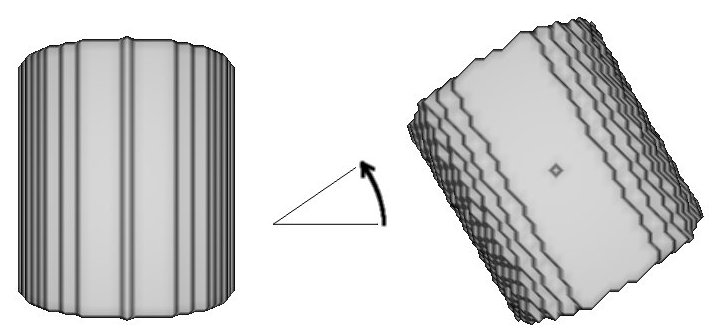
\includegraphics[width=8cm]{images/op_rotate.jpg}}}
  \\
  \hline
  
  \textbf{Skalowanie}
  Skaluje obiekt, na rzecz którego następuje wywołanie o podaną wartość wzdłuż
  osi X, Y, Z &
  local cube = Cube(); \newline cube:scale(1, 0.5, 1) \newline
  -- skaluje obiekt do połowy jego oryginalnego wymiaru wzdłuż osi Y; \\ \hline
  \multicolumn{2}{|c|}{\fbox{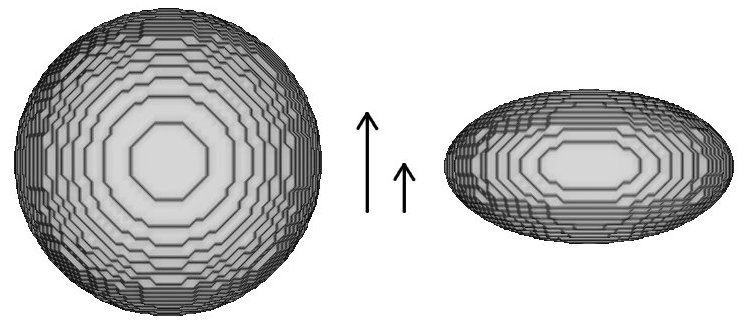
\includegraphics[width=8cm]{images/op_scale.jpg}}}
  \\
  \hline
\end{tabular}
\caption{Transformacje na obiektach elementarnych (zobacz~\ref{elements_table})
dostępne w gramatyce kształtu (źródło własne)}
\label{transforms_table}
\end{table}
\end{center}
}

{
\noindent
\begin{center}
\begin{table}[hp]
\begin{tabular}{| p{0.40\textwidth} | p{0.50\textwidth} | }
  \hline
  \rowcolor{lightgray} Typ operacji & Przykład użycia \\ \hline \hline
  
  \textbf{Suma elememtów} &
  local op = Or(sphere, cylinder); \newline draw(op); \\ \hline
  \multicolumn{2}{|c|}{\fbox{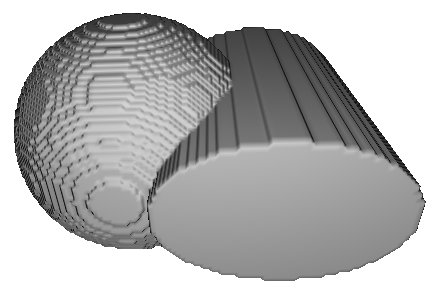
\includegraphics[height=4cm]{images/logic_or.jpg}}}
  \\
  \hline
  
  \textbf{Część wspólna} &
  local op = And(sphere, cylinder); \newline draw(op); \\ \hline
  \multicolumn{2}{|c|}{\fbox{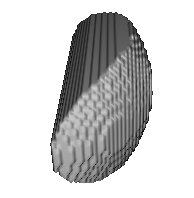
\includegraphics[height=4cm]{images/logic_and.jpg}}}
  \\
  \hline
  
  \textbf{Różnica} &
  local op = Diff(sphere, cylinder); \newline draw(op); \\ \hline
  \multicolumn{2}{|c|}{\fbox{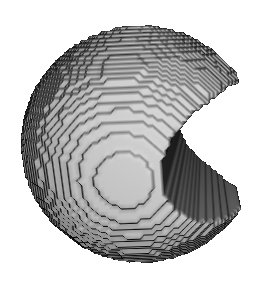
\includegraphics[height=4cm]{images/logic_diff.jpg}}}
  \\
  \hline
  
  \textbf{Różnica symetryczna}, w przykładzie przekrój modelu po wykonanej
  operacji Xor &
  local op = Xor(sphere, cylinder); \newline draw(op); \\ \hline
  \multicolumn{2}{|c|}{\fbox{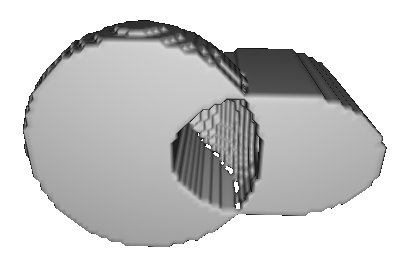
\includegraphics[height=4cm]{images/logic_xor.jpg}}}
  \\
  \hline
\end{tabular}
\caption{Operacje logiczne na obiektach elementarnych
(zobacz~\ref{elements_table}) dostępne z poziomu gramatyki kształtu (źródło
własne)}
\label{operations_table}
\end{table}
\end{center}
}

{
\noindent
\begin{center}
\begin{table}[hp]
\begin{tabular}{| p{0.50\textwidth} | p{0.4\textwidth} | }
  \hline
  \rowcolor{lightgray} Opis obiektu & Przykład użycia \\ \hline \hline
  
  \textbf{Odbicie lustrzane}\newline
  Generuje kopię elementu odbitą względem osi X, Y lub Z. Drugi parametr w
  konstruktorze obiektu Mirror oznacza oś odbicia przyjmując, że 0 - oś X, 1 -
  oś Y, 2 - oś Z &
  local elem = Cube(); \newline elem scale(0.3, 0.3, 0.3); \newline
  elem translate(-1.2, 0, 0); \newline local mirror = Mirror(elem, 0); \newline
  local both = Or(elem, mirror); \newline draw(both); \\ \hline
  \multicolumn{2}{|c|}{\fbox{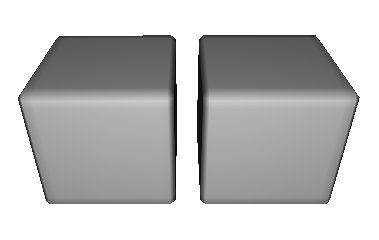
\includegraphics[height=4cm]{images/misc_mirror.jpg}}}
  \\
  \hline

  \textbf{Płaszczyzna}
  \newline Tworzy płaszczyznę, której normalna jest wektorem (1, 0, 0). &
  local cylinder = Cylinder(); \newline cylinder:scale(0.6, 0.6, 0.6); \newline
  local plane = Plane(); \newline plane:rotateDeg(0, -15, 0); \newline local op
  = And(cylinder, plane); \newline draw(op); \\ \hline
  \multicolumn{2}{|c|}{\fbox{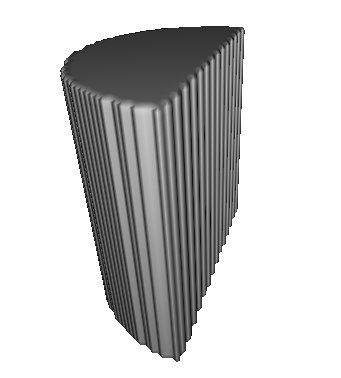
\includegraphics[height=4cm]{images/misc_plane.jpg}}}
  \\
  \hline
  
  \textbf{Dostęp do parametrów}
  \newline Aby w skrypcie gramatyki uzyskać dostęp do parametrów
  zdefiniowanych w programie należy skorzystać z metod klasy \emph{params}
  podając nazwę parametru. &
  local floatParam = params:getParamFloat(``Nazwa''); \newline local intParam
  = params:getParamInt(``Nazwa 1''); \newline local stringParam =
  params:getParamString(``Nazwa 2'');
  \\
  \hline
\end{tabular}
\caption{Dodatkowe operacje i modyfikatory (źródło własne)}
\label{misc_table}
\end{table}
\end{center}
}

{
\noindent
\begin{center}
\begin{table}[!htbp]
\begin{tabular}{| p{0.50\textwidth} | p{0.4\textwidth} | }
  \hline
  \rowcolor{lightgray} Opis obiektu & Przykład użycia \\ \hline \hline
  
  \textbf{Modyfikator płaszczyzny}
  \newline Tworzy płaszczyznę ,,odpychającą'' woksele. Domyślna normalna
  powierzchni jest wektorem (1, 0, 0). Jako parametr konstruktora należy podać
  modyfikowany obiekt gramatyki, zasięg działania modyfikatora oraz
  siłę odpychania (maleje wraz ze wzrostem odległości punktu od powierzchni). Do
  modyfikowania położenia, orientacji i skali powierzchni należy używać metod z
  przedrostkiem \emph{p\_} np. \emph{p\_rotateDeg(10, 0, 0)}. & local sphere =
  Sphere(); \newline local mod = PlaneProp(sphere, 1, 0.5); \newline mod:p\_rotateDeg(0, 180, 0); \newline mod:p\_translate(1, 0, 0); \newline draw(mod); \\ \hline
  \multicolumn{2}{|c|}{\fbox{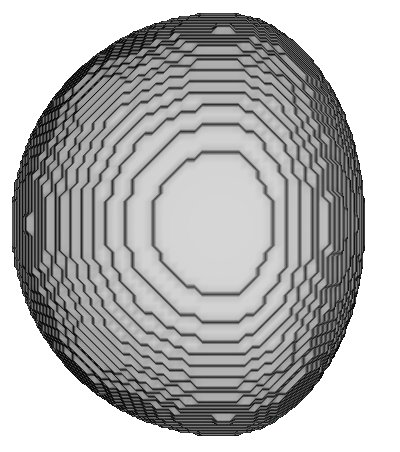
\includegraphics[height=4cm]{images/op_push.jpg}}}
  \\
  \hline
\end{tabular}
\caption{Dodatkowe operacje i modyfikatory cd. (źródło własne)}
\label{misc_table1}
\end{table}
\end{center}
}
